\documentclass{standalone}
\usepackage{tikz}
\usetikzlibrary{patterns, positioning}
\usepackage[sfdefault]{ClearSans} %% option 'sfdefault' activates Clear Sans as the default text font
\usepackage[T1]{fontenc}

\begin{document}
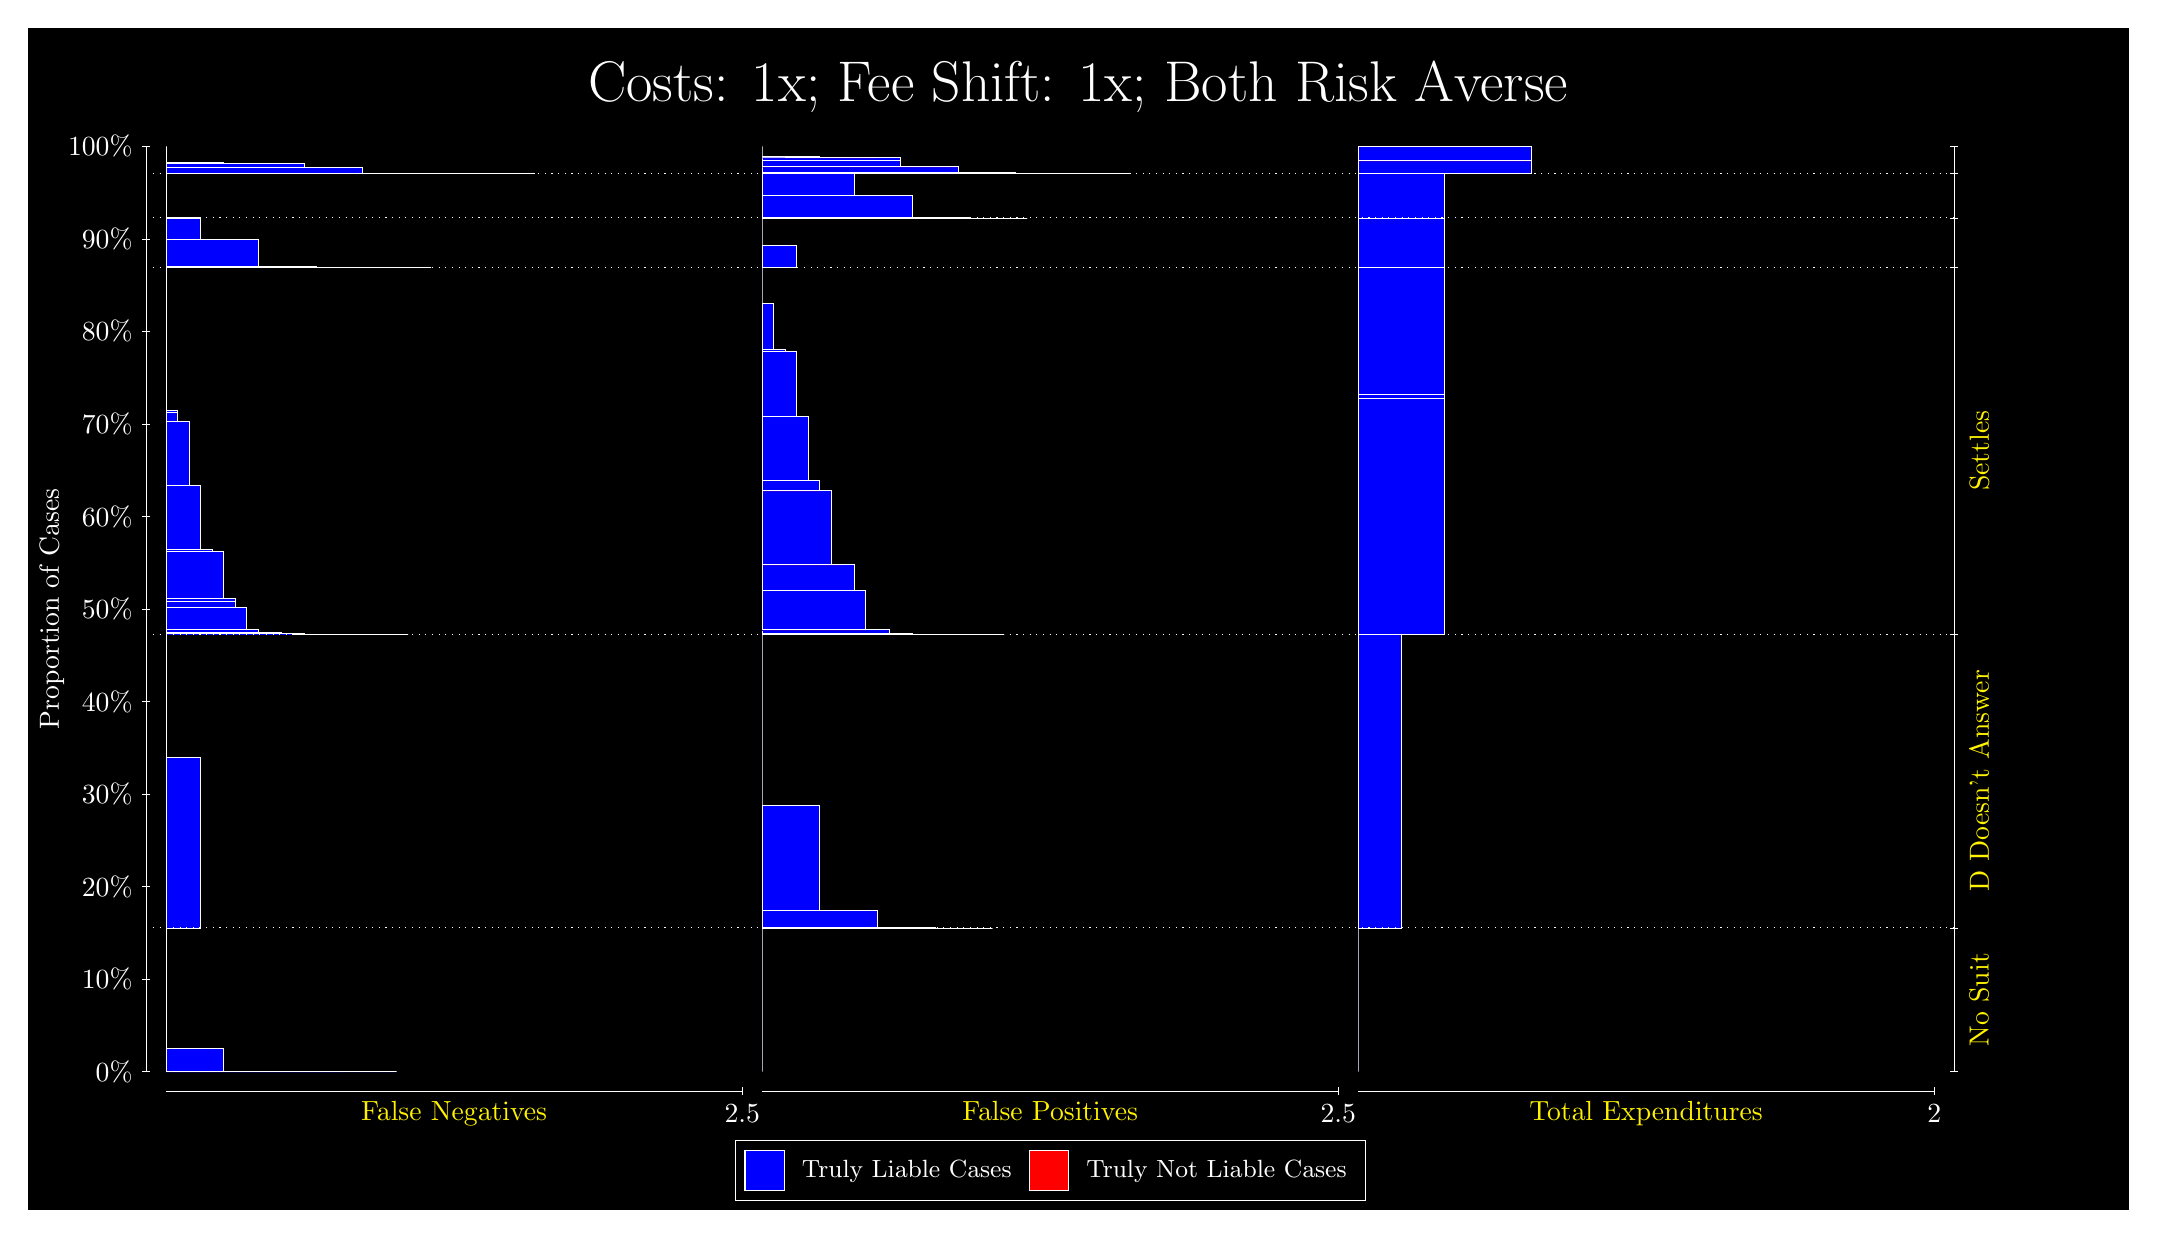
\begin{tikzpicture}
\draw[fill=black] (0,0) rectangle (26.667,15);
\draw[text=white] (0,13.5) rectangle (26.667,15) node[midway] {\huge Costs: 1x; Fee Shift: 1x; Both Risk Averse};
\draw[white, very thin] (1.5,1.75) -- (1.5,13.5);
\node[rotate=90, text=white, anchor=center] at (0.3, 7.625) {Proportion of Cases};
\draw[white, very thin] (1.45,1.75) -- (1.55,1.75);
\node[text=white, anchor=east] at (1.45, 1.75) {0\%};
\draw[white, very thin] (1.45,2.925) -- (1.55,2.925);
\node[text=white, anchor=east] at (1.45, 2.925) {10\%};
\draw[white, very thin] (1.45,4.1) -- (1.55,4.1);
\node[text=white, anchor=east] at (1.45, 4.1) {20\%};
\draw[white, very thin] (1.45,5.275) -- (1.55,5.275);
\node[text=white, anchor=east] at (1.45, 5.275) {30\%};
\draw[white, very thin] (1.45,6.45) -- (1.55,6.45);
\node[text=white, anchor=east] at (1.45, 6.45) {40\%};
\draw[white, very thin] (1.45,7.625) -- (1.55,7.625);
\node[text=white, anchor=east] at (1.45, 7.625) {50\%};
\draw[white, very thin] (1.45,8.8) -- (1.55,8.8);
\node[text=white, anchor=east] at (1.45, 8.8) {60\%};
\draw[white, very thin] (1.45,9.975) -- (1.55,9.975);
\node[text=white, anchor=east] at (1.45, 9.975) {70\%};
\draw[white, very thin] (1.45,11.15) -- (1.55,11.15);
\node[text=white, anchor=east] at (1.45, 11.15) {80\%};
\draw[white, very thin] (1.45,12.325) -- (1.55,12.325);
\node[text=white, anchor=east] at (1.45, 12.325) {90\%};
\draw[white, very thin] (1.45,13.5) -- (1.55,13.5);
\node[text=white, anchor=east] at (1.45, 13.5) {100\%};

\draw[white, very thin] (24.457,1.75) -- (24.457,13.5);
\draw[white, very thin] (24.407,1.75) -- (24.507,1.75);
\node[anchor=west] at (24.407, 1.75) {};
\draw[white, very thin] (24.407,3.5742) -- (24.507,3.5742);
\node[anchor=west] at (24.407, 3.5742) {};
\draw[white, very thin] (24.407,7.3049) -- (24.507,7.3049);
\node[anchor=west] at (24.407, 7.3049) {};
\draw[white, very thin] (24.407,11.965) -- (24.507,11.965);
\node[anchor=west] at (24.407, 11.965) {};
\draw[white, very thin] (24.407,12.591) -- (24.507,12.591);
\node[anchor=west] at (24.407, 12.591) {};
\draw[white, very thin] (24.407,13.158) -- (24.507,13.158);
\node[anchor=west] at (24.407, 13.158) {};
\draw[white, very thin] (24.407,13.5) -- (24.507,13.5);
\node[anchor=west] at (24.407, 13.5) {};

\draw[white, very thin, fill=blue] (1.75,1.75) rectangle (4.6775,1.75);
\draw[white, very thin, fill=blue] (1.75,1.75) rectangle (3.9457,1.75);
\draw[white, very thin, fill=blue] (1.75,1.75) rectangle (3.2138,1.7526);
\draw[white, very thin, fill=blue] (1.75,1.7526) rectangle (2.4819,2.0487);
\draw[white, very thin, fill=red] (1.75,2.0487) rectangle (1.75,2.0487);
\draw[white, very thin, fill=blue] (1.75,2.0487) rectangle (1.75,3.5742);
\draw[white, very thin, fill=blue] (1.75,3.5742) rectangle (2.1891,5.7446);
\draw[white, very thin, fill=red] (1.75,5.7446) rectangle (1.75,5.7446);
\draw[white, very thin, fill=blue] (1.75,5.7446) rectangle (1.75,7.3049);
\draw[white, very thin, fill=blue] (1.75,7.3049) rectangle (4.8239,7.3049);
\draw[white, very thin, fill=blue] (1.75,7.3049) rectangle (4.5312,7.3049);
\draw[white, very thin, fill=blue] (1.75,7.3049) rectangle (4.2384,7.3049);
\draw[white, very thin, fill=blue] (1.75,7.3049) rectangle (4.092,7.3049);
\draw[white, very thin, fill=blue] (1.75,7.3049) rectangle (3.9457,7.3049);
\draw[white, very thin, fill=blue] (1.75,7.3049) rectangle (3.7993,7.3049);
\draw[white, very thin, fill=blue] (1.75,7.3049) rectangle (3.6529,7.3049);
\draw[white, very thin, fill=blue] (1.75,7.3049) rectangle (3.5065,7.3113);
\draw[white, very thin, fill=blue] (1.75,7.3113) rectangle (3.3602,7.3123);
\draw[white, very thin, fill=blue] (1.75,7.3123) rectangle (3.2138,7.3263);
\draw[white, very thin, fill=blue] (1.75,7.3263) rectangle (3.0674,7.3263);
\draw[white, very thin, fill=blue] (1.75,7.3263) rectangle (3.0674,7.3271);
\draw[white, very thin, fill=blue] (1.75,7.3271) rectangle (2.921,7.3627);
\draw[white, very thin, fill=blue] (1.75,7.3627) rectangle (2.7746,7.6402);
\draw[white, very thin, fill=blue] (1.75,7.6402) rectangle (2.6283,7.7268);
\draw[white, very thin, fill=blue] (1.75,7.7268) rectangle (2.6283,7.7583);
\draw[white, very thin, fill=blue] (1.75,7.7583) rectangle (2.4819,8.3514);
\draw[white, very thin, fill=blue] (1.75,8.3514) rectangle (2.3355,8.3627);
\draw[white, very thin, fill=blue] (1.75,8.3627) rectangle (2.3355,8.3764);
\draw[white, very thin, fill=blue] (1.75,8.3764) rectangle (2.1891,9.1932);
\draw[white, very thin, fill=blue] (1.75,9.1932) rectangle (2.0428,10.009);
\draw[white, very thin, fill=blue] (1.75,10.009) rectangle (1.8964,10.118);
\draw[white, very thin, fill=blue] (1.75,10.118) rectangle (1.8964,10.143);
\draw[white, very thin, fill=red] (1.75,10.143) rectangle (1.75,10.143);
\draw[white, very thin, fill=blue] (1.75,10.143) rectangle (1.75,11.965);
\draw[white, very thin, fill=blue] (1.75,11.965) rectangle (5.1167,11.965);
\draw[white, very thin, fill=blue] (1.75,11.965) rectangle (4.3848,11.965);
\draw[white, very thin, fill=blue] (1.75,11.965) rectangle (3.6529,11.973);
\draw[white, very thin, fill=blue] (1.75,11.973) rectangle (2.921,12.318);
\draw[white, very thin, fill=blue] (1.75,12.318) rectangle (2.1891,12.591);
\draw[white, very thin, fill=red] (1.75,12.591) rectangle (1.75,12.591);
\draw[white, very thin, fill=blue] (1.75,12.591) rectangle (2.1891,12.595);
\draw[white, very thin, fill=red] (1.75,12.595) rectangle (1.75,12.595);
\draw[white, very thin, fill=blue] (1.75,12.595) rectangle (1.75,13.158);
\draw[white, very thin, fill=blue] (1.75,13.158) rectangle (6.4341,13.158);
\draw[white, very thin, fill=blue] (1.75,13.158) rectangle (5.7022,13.158);
\draw[white, very thin, fill=blue] (1.75,13.158) rectangle (4.9703,13.163);
\draw[white, very thin, fill=blue] (1.75,13.163) rectangle (4.2384,13.232);
\draw[white, very thin, fill=blue] (1.75,13.232) rectangle (3.9457,13.232);
\draw[white, very thin, fill=blue] (1.75,13.232) rectangle (3.5065,13.29);
\draw[white, very thin, fill=blue] (1.75,13.29) rectangle (3.2138,13.29);
\draw[white, very thin, fill=blue] (1.75,13.29) rectangle (2.7746,13.291);
\draw[white, very thin, fill=blue] (1.75,13.291) rectangle (2.4819,13.3);
\draw[white, very thin, fill=blue] (1.75,13.3) rectangle (2.0428,13.3);
\draw[white, very thin, fill=red] (1.75,13.3) rectangle (1.75,13.3);
\draw[white, very thin, fill=blue] (1.75,13.3) rectangle (1.75,13.5);
\draw[white, very thin, fill=red] (9.3189,1.75) rectangle (9.3189,1.75);
\draw[white, very thin, fill=blue] (9.3189,1.75) rectangle (9.3189,3.5742);
\draw[white, very thin, fill=red] (9.3189,3.5742) rectangle (12.246,3.5742);
\draw[white, very thin, fill=blue] (9.3189,3.5742) rectangle (12.246,3.5742);
\draw[white, very thin, fill=blue] (9.3189,3.5742) rectangle (11.515,3.5758);
\draw[white, very thin, fill=blue] (9.3189,3.5758) rectangle (10.783,3.8004);
\draw[white, very thin, fill=blue] (9.3189,3.8004) rectangle (10.051,5.1345);
\draw[white, very thin, fill=blue] (9.3189,5.1345) rectangle (9.3189,7.3049);
\draw[white, very thin, fill=red] (9.3189,7.3049) rectangle (12.393,7.3049);
\draw[white, very thin, fill=blue] (9.3189,7.3049) rectangle (12.393,7.3049);
\draw[white, very thin, fill=red] (9.3189,7.3049) rectangle (11.807,7.3049);
\draw[white, very thin, fill=blue] (9.3189,7.3049) rectangle (11.807,7.3049);
\draw[white, very thin, fill=blue] (9.3189,7.3049) rectangle (11.661,7.3049);
\draw[white, very thin, fill=red] (9.3189,7.3049) rectangle (11.515,7.3049);
\draw[white, very thin, fill=blue] (9.3189,7.3049) rectangle (11.515,7.3049);
\draw[white, very thin, fill=red] (9.3189,7.3049) rectangle (11.222,7.3049);
\draw[white, very thin, fill=blue] (9.3189,7.3049) rectangle (11.222,7.3165);
\draw[white, very thin, fill=blue] (9.3189,7.3165) rectangle (11.075,7.3165);
\draw[white, very thin, fill=red] (9.3189,7.3165) rectangle (10.929,7.3165);
\draw[white, very thin, fill=blue] (9.3189,7.3165) rectangle (10.929,7.3609);
\draw[white, very thin, fill=blue] (9.3189,7.3609) rectangle (10.783,7.362);
\draw[white, very thin, fill=red] (9.3189,7.362) rectangle (10.636,7.362);
\draw[white, very thin, fill=blue] (9.3189,7.362) rectangle (10.636,7.8563);
\draw[white, very thin, fill=blue] (9.3189,7.8563) rectangle (10.49,8.186);
\draw[white, very thin, fill=red] (9.3189,8.186) rectangle (10.344,8.186);
\draw[white, very thin, fill=blue] (9.3189,8.186) rectangle (10.344,8.1983);
\draw[white, very thin, fill=blue] (9.3189,8.1983) rectangle (10.197,9.1265);
\draw[white, very thin, fill=red] (9.3189,9.1265) rectangle (10.051,9.1265);
\draw[white, very thin, fill=blue] (9.3189,9.1265) rectangle (10.051,9.2604);
\draw[white, very thin, fill=blue] (9.3189,9.2604) rectangle (9.9044,10.076);
\draw[white, very thin, fill=blue] (9.3189,10.076) rectangle (9.758,10.893);
\draw[white, very thin, fill=blue] (9.3189,10.893) rectangle (9.6116,10.918);
\draw[white, very thin, fill=blue] (9.3189,10.918) rectangle (9.4652,11.511);
\draw[white, very thin, fill=blue] (9.3189,11.511) rectangle (9.3189,11.965);
\draw[white, very thin, fill=red] (9.3189,11.965) rectangle (9.758,11.965);
\draw[white, very thin, fill=blue] (9.3189,11.965) rectangle (9.758,12.238);
\draw[white, very thin, fill=blue] (9.3189,12.238) rectangle (9.3189,12.591);
\draw[white, very thin, fill=red] (9.3189,12.591) rectangle (12.686,12.591);
\draw[white, very thin, fill=blue] (9.3189,12.591) rectangle (12.686,12.591);
\draw[white, very thin, fill=blue] (9.3189,12.591) rectangle (11.954,12.595);
\draw[white, very thin, fill=blue] (9.3189,12.595) rectangle (11.222,12.876);
\draw[white, very thin, fill=blue] (9.3189,12.876) rectangle (10.49,13.155);
\draw[white, very thin, fill=blue] (9.3189,13.155) rectangle (9.758,13.158);
\draw[white, very thin, fill=red] (9.3189,13.158) rectangle (14.003,13.158);
\draw[white, very thin, fill=blue] (9.3189,13.158) rectangle (14.003,13.158);
\draw[white, very thin, fill=red] (9.3189,13.158) rectangle (13.271,13.158);
\draw[white, very thin, fill=blue] (9.3189,13.158) rectangle (13.271,13.158);
\draw[white, very thin, fill=red] (9.3189,13.158) rectangle (12.539,13.158);
\draw[white, very thin, fill=blue] (9.3189,13.158) rectangle (12.539,13.165);
\draw[white, very thin, fill=blue] (9.3189,13.165) rectangle (11.807,13.243);
\draw[white, very thin, fill=red] (9.3189,13.243) rectangle (11.807,13.243);
\draw[white, very thin, fill=blue] (9.3189,13.243) rectangle (11.807,13.243);
\draw[white, very thin, fill=blue] (9.3189,13.243) rectangle (11.075,13.319);
\draw[white, very thin, fill=blue] (9.3189,13.319) rectangle (11.075,13.358);
\draw[white, very thin, fill=red] (9.3189,13.358) rectangle (10.783,13.358);
\draw[white, very thin, fill=blue] (9.3189,13.358) rectangle (10.783,13.358);
\draw[white, very thin, fill=blue] (9.3189,13.358) rectangle (10.344,13.358);
\draw[white, very thin, fill=blue] (9.3189,13.358) rectangle (10.344,13.367);
\draw[white, very thin, fill=red] (9.3189,13.367) rectangle (10.051,13.367);
\draw[white, very thin, fill=blue] (9.3189,13.367) rectangle (10.051,13.368);
\draw[white, very thin, fill=blue] (9.3189,13.368) rectangle (9.6116,13.368);
\draw[white, very thin, fill=blue] (9.3189,13.368) rectangle (9.6116,13.368);
\draw[white, very thin, fill=red] (9.3189,13.368) rectangle (9.3189,13.368);
\draw[white, very thin, fill=blue] (9.3189,13.368) rectangle (9.3189,13.5);
\draw[white, very thin, fill=red] (16.888,1.75) rectangle (16.888,1.75);
\draw[white, very thin, fill=blue] (16.888,1.75) rectangle (16.888,3.5742);
\draw[white, very thin, fill=red] (16.888,3.5742) rectangle (17.437,3.5742);
\draw[white, very thin, fill=blue] (16.888,3.5742) rectangle (17.437,7.3049);
\draw[white, very thin, fill=red] (16.888,7.3049) rectangle (17.986,7.3049);
\draw[white, very thin, fill=blue] (16.888,7.3049) rectangle (17.986,10.298);
\draw[white, very thin, fill=red] (16.888,10.298) rectangle (17.986,10.298);
\draw[white, very thin, fill=blue] (16.888,10.298) rectangle (17.986,10.355);
\draw[white, very thin, fill=red] (16.888,10.355) rectangle (17.986,10.355);
\draw[white, very thin, fill=blue] (16.888,10.355) rectangle (17.986,11.965);
\draw[white, very thin, fill=red] (16.888,11.965) rectangle (17.986,11.965);
\draw[white, very thin, fill=blue] (16.888,11.965) rectangle (17.986,12.591);
\draw[white, very thin, fill=red] (16.888,12.591) rectangle (17.986,12.591);
\draw[white, very thin, fill=blue] (16.888,12.591) rectangle (17.986,13.158);
\draw[white, very thin, fill=red] (16.888,13.158) rectangle (19.083,13.158);
\draw[white, very thin, fill=blue] (16.888,13.158) rectangle (19.083,13.319);
\draw[white, very thin, fill=red] (16.888,13.319) rectangle (19.083,13.319);
\draw[white, very thin, fill=blue] (16.888,13.319) rectangle (19.083,13.5);
\draw[white, dotted] (1.5,3.5742) -- (24.457,3.5742);
\draw[white, dotted] (1.5,7.3049) -- (24.457,7.3049);
\draw[white, dotted] (1.5,11.965) -- (24.457,11.965);
\draw[white, dotted] (1.5,12.591) -- (24.457,12.591);
\draw[white, dotted] (1.5,13.158) -- (24.457,13.158);
\draw[white, very thin] (1.75,1.5) -- (9.0689,1.5);
\node[text=yellow, anchor=north] at (5.4094, 1.5) {False Negatives};
\draw[white, very thin] (9.0689,1.45) -- (9.0689,1.55);
\node[text=white, anchor=north] at (9.0689, 1.45) {2.5};

\draw[white, very thin] (9.3189,1.5) -- (16.638,1.5);
\node[text=yellow, anchor=north] at (12.978, 1.5) {False Positives};
\draw[white, very thin] (16.638,1.45) -- (16.638,1.55);
\node[text=white, anchor=north] at (16.638, 1.45) {2.5};

\draw[white, very thin] (16.888,1.5) -- (24.207,1.5);
\node[text=yellow, anchor=north] at (20.547, 1.5) {Total Expenditures};
\draw[white, very thin] (24.207,1.45) -- (24.207,1.55);
\node[text=white, anchor=north] at (24.207, 1.45) {2};

\node[text=yellow, centered, rotate=90] at (24.777, 2.6621) {No Suit};
\node[text=yellow, centered, rotate=90] at (24.777, 5.4396) {D Doesn't Answer};
\node[text=yellow, centered, rotate=90] at (24.777, 9.6348) {Settles};




\draw (12.978300999999998,1.5) node[draw=none] (baseCoordinate) {};
\begin{scope}[align=center]
        \matrix[scale=0.5, draw=white, below=0.5cm of baseCoordinate, nodes={draw}, column sep=0.1cm]{
            \node[rectangle, draw, minimum width=0.5cm, minimum height=0.5cm, fill=blue] {}; &
            \node[draw=none, font=\small, text=white] (B) {Truly Liable Cases}; &
            \node[rectangle, draw, minimum width=0.5cm, minimum height=0.5cm, fill=red] {}; &
            \node[draw=none, font=\small, text=white] (B) {Truly Not Liable Cases}; \\
            };
\end{scope}

\end{tikzpicture}
\end{document}